\chapter{Anatomische Segmentierung}
\label{chap:theoretische_grundlagen} Die anatomische Segmentierung ist ein bestehendes
Verfahren, das bereits von der Klinik an der LMU eingesetzt wird, um segmentierte
Daten aus Mikro-\ac{CT}-Bildern gezielt zu gewinnen. Einen wichtigen Meilenstein
hierfür liefert Hofmann. Im Rahmen einer Bachelorarbeit an der Hochschule für
angewandte Wissenschaften in Augsburg unterstützte Herr Hofmann die
Kariesklassifizierung auf den Zahnkronen-\ac{CT}-Aufnahmen. Hierzu entwickelte
er ein Verfahren, das auf Basis von Schwellwertverfahren die Zahnsubstanzen Schmelz
und Dentin aus dem Originalbild herauslöst. Dabei wird die anatomische
Segmentierung als der Prozess verstanden, bei dem diese Gewebetypen gezielt voneinander
getrennt und visuell sowie rechnerisch unterscheidbar gemacht werden.

\begin{minipage}{0.40\textwidth}
	Durch die Segmentbetrachtung der beiden Gewebesubstanzen Schmelz und Dentin konnte
	\citet[S.~41]{hoffmann2020} eine gute Hilfe für die Befundung kariöse Stellen
	liefern. Ein Ergebnis aus der Arbeit von Hofmann sei in Abbildung \ref{fig:ergebnis_hoffmann}
	gezeigt. Hierfür entwickelte Hofmann ein prototypisches Verfahren innerhalb
	eines IPython Notebooks, mit dem es gelang ca. 250 Datensätze der Klinik
	automatisch aufzubereiten.
\end{minipage}
\hfill
\begin{minipage}{0.50\textwidth}
	\centering
	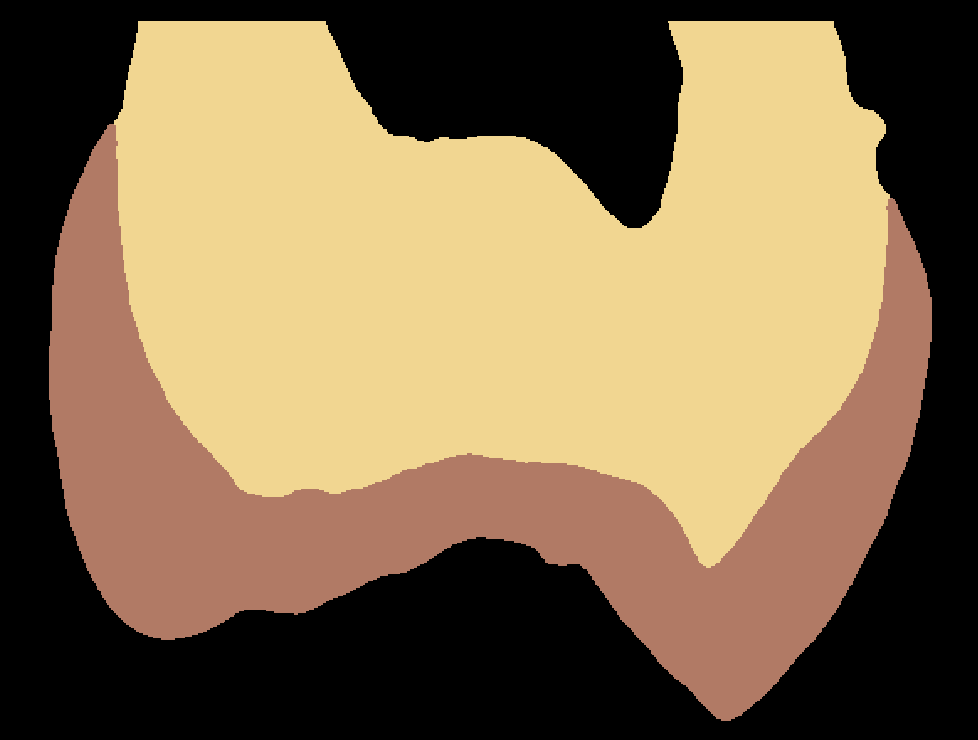
\includegraphics[width=0.7\textwidth]{img/ergebnis_hoffmann_2.jpg}
	\captionof{figure}{Reproduziertes Ergebnis der anatomischen Segmentierung} \label{fig:ergebnis_hoffmann}
\end{minipage}

Neben der Erstellung von segmentierten Daten stellt das Verfahren noch
sogenannte mediale Flächen zur Verfügung. Diese sind insbesondere für die Klassifizierung
von Karies notwendig. \citet[S.~42]{hoffmann2020} erklärt, das sich bei einer
Überlagert der medialen Flächen auf das Originale Bild auf einem Blick erkennen
lassen, ob die vorhandene Karies in diesen Schichten weiter als die Hälfte fortgeschritten
ist. Für die Erstellung der medial Flächen sind die segmentierte Daten eines
Zahnes zwingend erforderlich. Die Berechnung der medial Flächen erfolgte auf den
Segmenten mithilfe einer Distanztransformation und anschließender Kantenfindung \citep[vgl.][S.~42]{hoffmann2020}.

Die anatomische Segmentierung eines Zahnes – einschließlich der medialen Flächen
– erfolgt in mehreren algorithmischen Schritten, die in einer klar strukturierten
Pipeline ablaufen. Abbildung \ref{fig:anatomische_segmentierung} veranschaulicht
den groben Ablauf des Verfahrens, wobei kleinere Zwischenschritte ausgeklammert sind.
Der Prozess beginnt oben links und endet mit der Segmentierung der medialen
Flächen in der unteren rechten Ecke.

\begin{figure}[h]
	\centering
	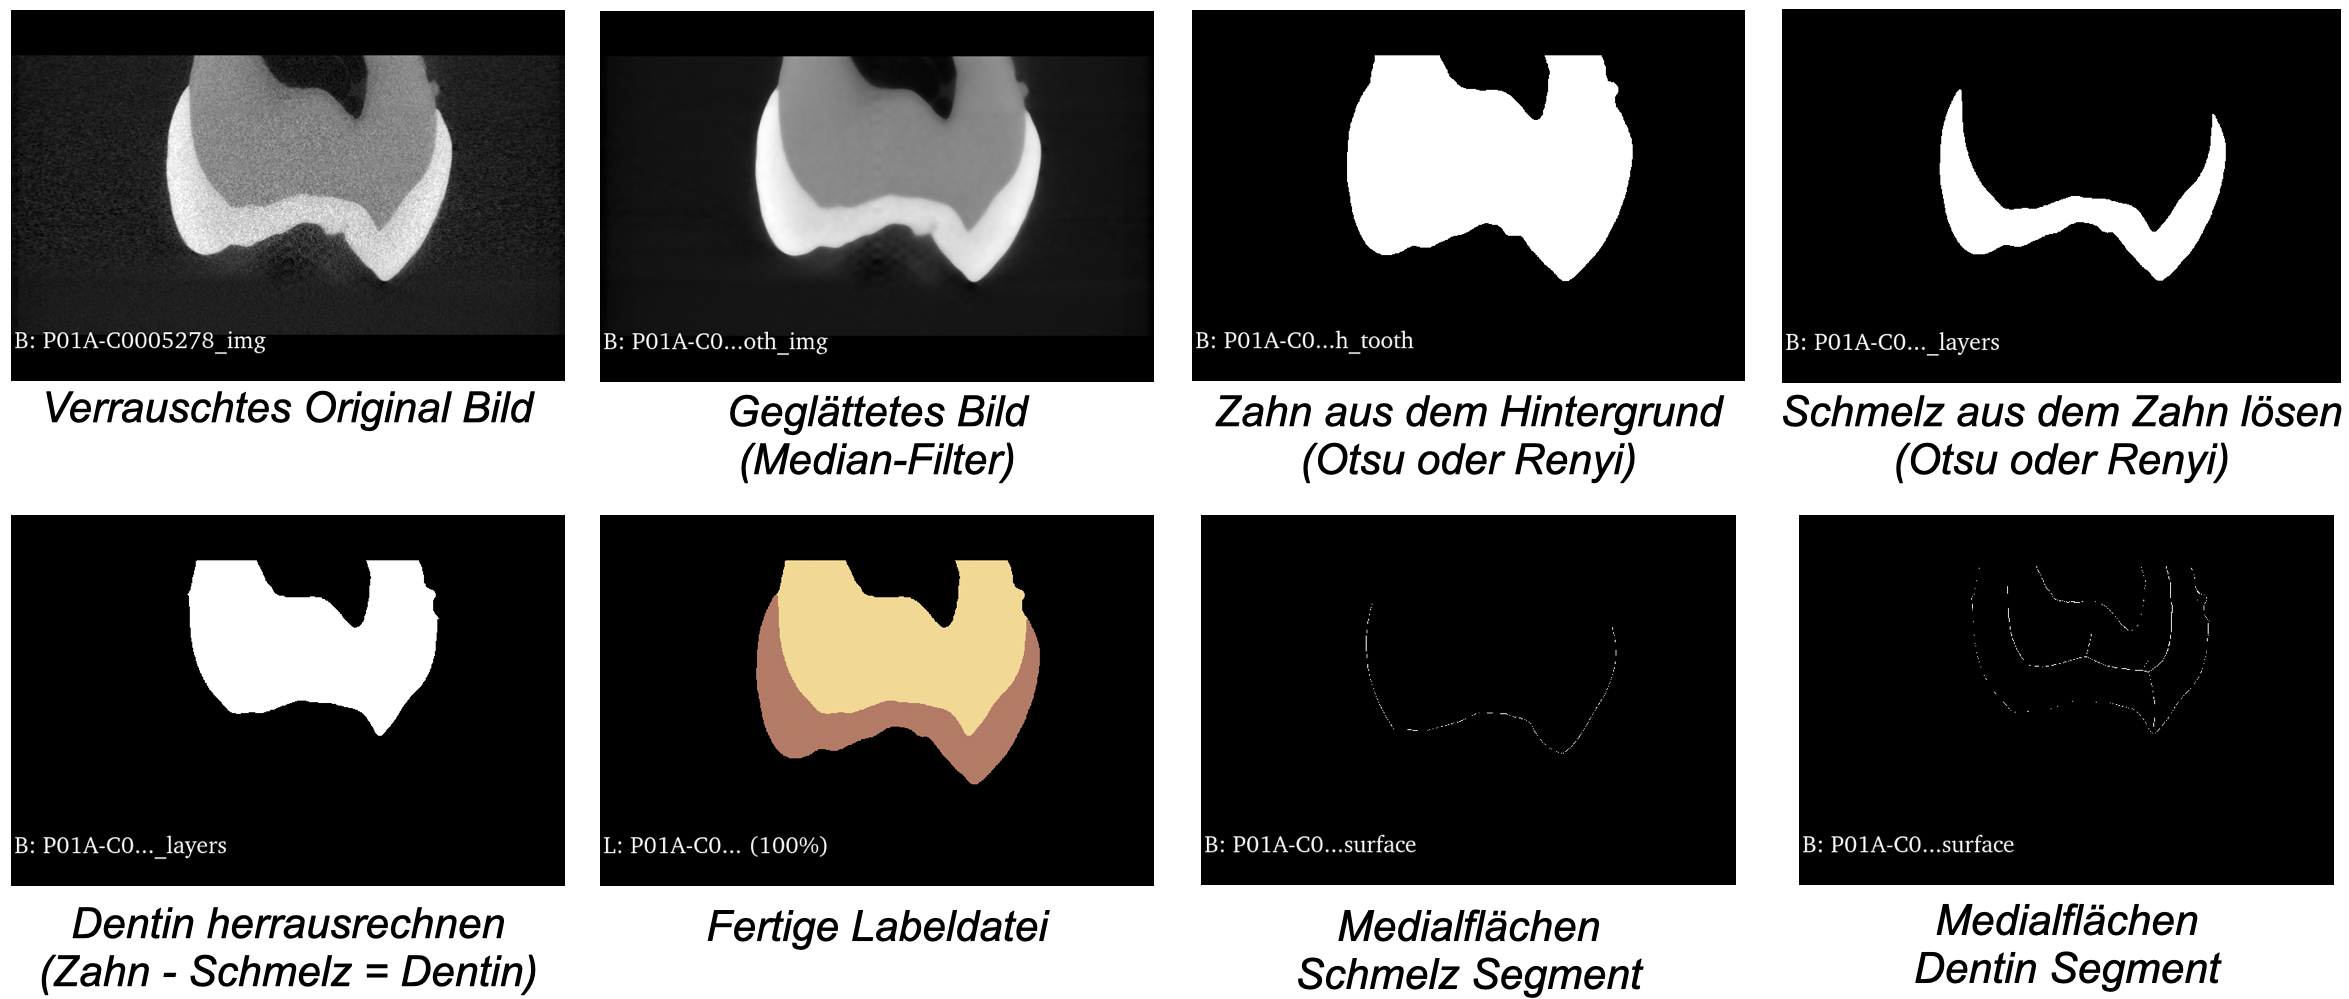
\includegraphics[width=1\textwidth]{img/anatomischeSegmentierung.png}
	\caption{Algorithmische Formulierung der anatomischen Segmentierung nach
	\citet{hoffmann2020} (von links oben nach rechts unten)}
	\label{fig:anatomische_segmentierung}
\end{figure}

Wie \citet[S.~55]{hoffmann2020} beschreibt, kann dieses Verfahren bis zu einem gewissen
Fortschritt von Karies angewendet werden. Da Karies im Laufe der Zeit zur
Zersetzung des Zahns führt, entstehen dunkle Stellen im Schmelzbereich, die die
zusammenhängenden Grauwerte im Bild stören und somit die Segmentierung
erschweren. Eine weitere Herausforderung liegt in der Art der Bilddaten, für die
das Verfahren ursprünglich entwickelt wurde. Es basiert auf \ac{ISQ}-Bildern, die
im \ac{16Int}-Format vorliegen.

Die einzelnen Schritte in Abbildung \ref{fig:anatomische_segmentierung}
verdeutlichen, dass die Segmentierung stets einem spezifischen Muster folgt und das
Verfahren primär zwischen Dentin und Schmelz unterscheidet. Die Pulpa wird wie
bereits beschrieben in diesem Verfahren nicht berücksichtigt. Zudem wird ersichtlich,
dass sowohl Filter als auch Segmentierungstechniken essenziell für eine präzise
Trennung der Strukturen sind. Um ein besseres Verständnis für diesen Prozess zu gewinnen,
führt das folgende Kapitel in die anatomischen Strukturen eines Zahns ein und
zeigt, wie diese auf Mikro-\ac{CT}-Aufnahmen erkennbar sind. Dabei werden die grundlegenden
Techniken der Bildgewinnung und -bearbeitung näher erläutert.

\pagebreak
% ---------------------------------------------------------------------------------------

\section{Anatomische Zahnstrukturen in Mikro-CT-Bildern}
\label{sec:domänenspezifisch} Um nachvollziehen zu können, wie eine \ac{CT}-Aufnahme
technisch segmentiert und in ihre einzelnen Bestandteile zerlegt werden kann,
ist es zunächst essenziell, die anatomische Struktur des Zahns genau zu verstehen.
Dazu gehören die unterschiedlichen Gewebeschichten wie Zahnschmelz, Dentin und die
Pulpa, die sich nicht nur in ihrer physikalischen Zusammensetzung, sondern auch in
ihrer radiologischen Darstellung innerhalb der \ac{CT}-Bilder unterscheiden. Erst
mit diesem grundlegenden Verständnis lassen sich Methoden zur \ac{3D}-Bildbearbeitung
ableiten.

\begin{minipage}{0.40\textwidth}
	Die Abbildung \ref{fig:aufbau_eines_zahnes} zeigt den groben Aufbau eines Zahnes
	nach \citet[S.~17]{lehmann2012Zahnheilkunde}. Zu sehen ist, dass das Denit
	oder auch Zahnbein genannt den Großteil eines Zahnes einnimmt. Im Bereich der Zahnkrone
	wird das Dentin von Zahnschmelz überzogen. Der Zahnschmelz ragt in die
	Mundhöhle und ist nach \citet[S.~41]{lehmann2012Zahnheilkunde} das härteste Material
	im menschlichen Körper. In der Mitte des Zahnes befindet sich Weichgewebe, das
	als Pulpa bezeichnet wird vgl. \citep[vgl.][S.~15]{lehmann2012Zahnheilkunde}.
	Für die anatomische Segmentierung von Zahn-\ac{CT}-Aufnahmen spielen insbesondere
	die drei Hauptbestandteile des Zahns – Schmelz, Dentin und Pulpa – eine
	entscheidende Rolle.
\end{minipage}
\hfill
\begin{minipage}{0.50\textwidth}
	\centering
	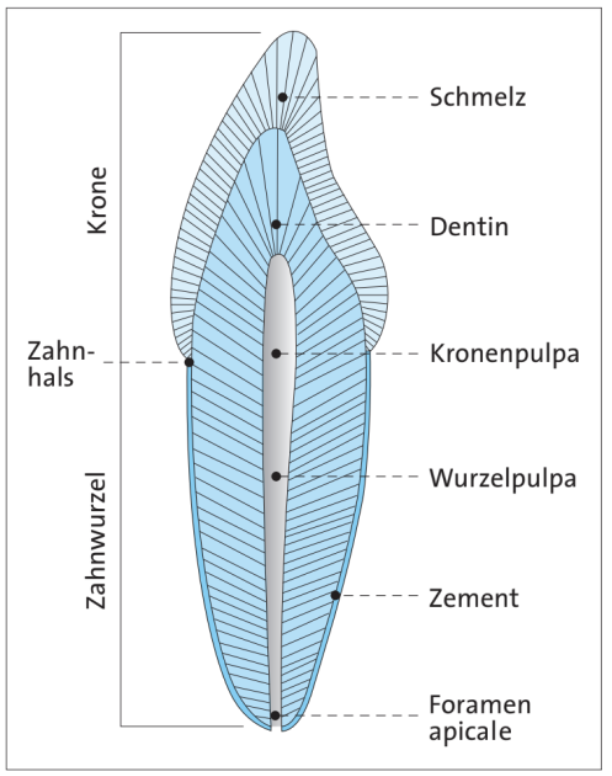
\includegraphics[scale=0.50]{img/aufbau_eines_zahns.jpg}
	\captionof{figure}{Aufbau eines ganzen Zahnes nach \citet[S.~15]{lehmann2012Zahnheilkunde}}
	\label{fig:aufbau_eines_zahnes}
\end{minipage}

Diese Gewebearten weisen unterschiedliche Strukturen auf, die sich in den
verschiedenen Graustufen auf einem Mikro-\ac{CT}-Bild widerspiegeln. Die Pulpa, das
innere Weichgewebe des Zahns, unterscheidet sich dabei nur geringfügig vom
Hintergrund, da sie als einzige der drei Hauptstrukturen nur sehr wenig Röntgenstrahlen
absorbiert. Aufgrund dieser geringen Sichtbarkeit spielt die Pulpa in dieser
Arbeit eine untergeordnete Rolle und wird nicht in das Segmentierungsverfahren
einbezogen. Geht man von innen nach außen, folgt auf die Pulpa das Dentin, das auch
als Zahnbein bezeichnet wird. Laut \citet[S.~41]{lehmann2012Zahnheilkunde} handelt
es sich dabei um eine Hartsubstanz, die den Zahn im Kieferknochen hält. Aufgrund
seiner Dichte ist das Dentin in \ac{CT}-Aufnahmen bereits deutlich erkennbar. Die
äußerste Schicht des Zahns bildet der Zahnschmelz. Dieser stellt die härteste
Substanz im menschlichen Körper dar und erscheint auf den \ac{CT}-Bildern besonders
hell. Seine hohe Dichte sorgt für eine klare Abgrenzung zu den darunterliegenden
Schichten, was ihn zu einem wichtigen Orientierungspunkt für die Segmentierung macht
\citep[vgl.][S.~41]{lehmann2012Zahnheilkunde}. Mit der folgenden Abbildung \ref{fig:pulpa_dentin_schmelz}
werden die verschiedenen Gewebearten in einem Zahn den entsprechenden Graustufen
zugeordnet.

\begin{figure}[h]
	\centering
	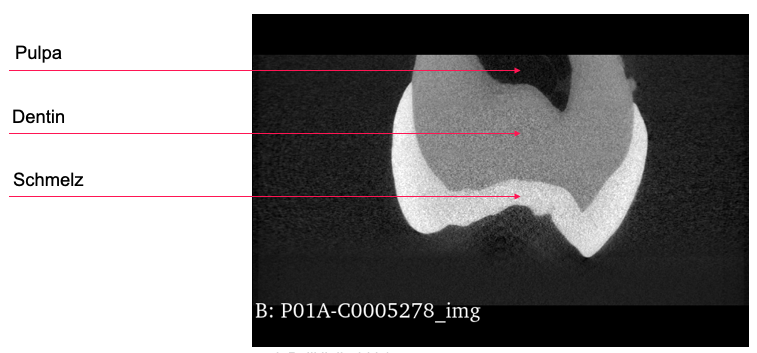
\includegraphics[width=0.9\textwidth]{img/dentin_schmelz_pulpa.png}
	\caption{Darstellung von Pulpa, Dentin und Schmelz auf einem Zahnkronen-CT nach
	\citet{heck2024}}
	\label{fig:pulpa_dentin_schmelz}
\end{figure}

Zu Beachten ist hier, dass es sich bei der in Abbildung \ref{fig:pulpa_dentin_schmelz}
gezeigten \ac{CT}-Aufnahme um eine Zahnkrone handelt und nicht um den ganzen
Zahn. Zu sehen ist auch der fast identische Grauwert zwischen dem Hintergrund und
der Pulpa.

Mit diesem Wissen über die Anatomie eines Zahnes und die Zusammensetzung auf einem
Mikro-\ac{CT}, kann nun ein Schritt weiter gegangen werden, indem der Fokus auf
die \ac{CT}-Bilder gerichtet wird. Das folgende Kapitel bietet daher einen
Überblick über die Erstellung von Röntgenaufnahmen sowie die Berechnung einer
Mikro-\ac{CT}-Aufnahme. Durch die Bildgewinnung wir auch klar, mit welcher hohen
Auflösung gearbeitet wird und warum dies auch zu Hindernissen führt.
% ---------------------------------------------------------------------------------------

\section{Erstellung von Mikro-CT-Bildern}
\label{sec:technologisch} Die Erzeugung dreidimensionaler Bilddaten ist ein essenzieller
Bestandteil der modernen medizinischen Bildgebung und kann auf verschiedene Weise
erfolgen. Je nach Anwendungsgebiet kommen unterschiedliche Verfahren zum Einsatz,
darunter \ac{MRT}, \ac{OCT} und insbesondere die Computertomografie \citep[vgl.][S.~14]{handels2000}.
Eine spezielle Variante der Computertomografie ist das Mikro-\ac{CT}, das durch
seine kleinere Ausführung in der zahnmedizinischen Forschung und Diagnostik eine
zentrale Rolle spielt. Auch die Handhabung dieser erstellten Daten ist ein wichtiger
Bestandteil der Forschung.
% ---------------------------------------------------------------------------------------

\subsection{Computertomografie}
\label{subsec:computertomografie} Die Erfindung der Computertomografie (\ac{CT})
war ein Quantensprung in der Geschichte der Medizin. Sie ist aus heutigen Diagnosen
nicht mehr wegzudenken. Ein Mikro-\ac{CT}-Bild ist laut \citet[S.~1]{baird2017}
ein Menge hochauflösender Bilder, die wie ein Stapel zusammengelegt werden.
Vereinfacht gesagt, werden so \ac{2D} Bilder zu einem \ac{3D}-\ac{CT}
zusammengesetzt. Der Aspekt Mikro deutet dabei darauf hin, dass es eine
miniaturisierte Ausführung eines üblichen Kegelstrahl-\ac{CT}s ist, so \citet[S.~340]{buzug2011}.
Eine andere Definition erläutert \citet[S.~49]{lehmann2013bildverarbeitung}. Er beschreibt
die Computertomografie als Projektionen einzelner Ebenen im Untersuchungsobjekt.
Die Abbildung \ref{fig:spectrum} soll diesen Vorgang genauer beschreiben.

\begin{figure}[h]
	\centering
	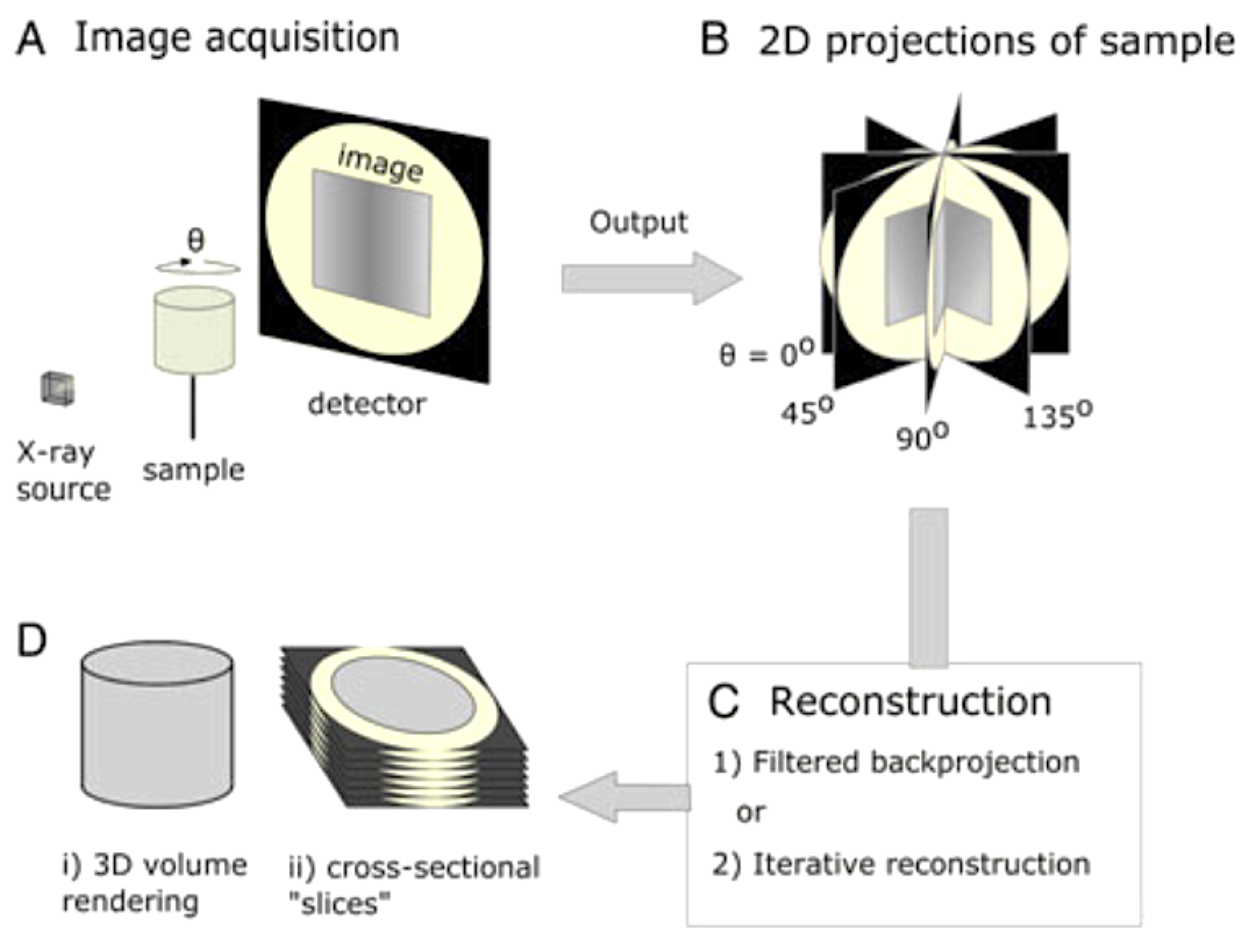
\includegraphics[width=0.6\textwidth]{img/Funktion_CT.png}
	\caption{Funktionsweise eines Mikro-CT nach \citet[S.~16]{pult2021}}
	\label{fig:spectrum}
\end{figure}

Die Technologie, mit der diese Bilder aufgenommen werden, ist unter der Röntgentechnik
oder auch \ac{X-Ray} bekannt. Die Röntgenstrahlung ist eine Form der elektromagnetischen
Strahlung, ähnlich wie das sichtbare Licht, so das \citet[K.~1]{nib2024}. Anders
als das Licht haben die Röntgenstrahlen eine viel höhere Energie. Das führt dazu,
dass man mit dieser elektromagnetischen Strahlung viele Objekte durchdringt werden
können. So auch Gewebeteile eines Zahnes \citep[vgl.][K.~1]{nib2024}. Mit der
Steigerung der Atomzahl in einem Material, also der Dichte, nimmt auch die
Absorption eines Materials zu, sodass es leicht ist verschiedene Materialien in einer
\ac{CT}-Aufnahme zu unterscheiden \citep[vgl.][K.~1]{nib2024}. Um nun mittels
der Röntgenstrahlen und den einzelnen \ac{2D} Projektionen ein \ac{3D}-Micro-\ac{CT}
zu erstellen, werden 2D-Röntgenaufnahmen eines Objektes aus verschiedenen
Winkeln geschossen und in einem weiteren Schritt dann zu einem \ac{3D}-Modell rekonstruiert.
Das Ergebnis einer solchen Rekonstruktion ist dann eine Art Papierstapel. Dieser
besteht aus vielen 2D-Bilder, die aufgrund der Stapelung zu einem \ac{3D}-Bild werden.

Für die Erzeugung dieser Bilder bedarf spezieller Geräte, im Falle der
Zahnklinik an der \ac{LMU} handelt es sich um ein Mikro-\ac{CT}-Gerät der Firma
\citet{scanco2024}. Dieses Gerät erstellt Aufnahmen mittels Röntgenstrahlung und
generiert mithilfe der Computertomografie ein dreidimensionales Bild, welches im
Format \ac{ISQ} abgelegt wird. Das folgende Kapitel zeigt, dass Mikro-\ac{CT}-Bilder
mit dem Typ \ac{ISQ} zwar eine hohe Detailgenauigkeit bieten, jedoch auch einen erheblichen
Speicherbedarf mit sich bringen.
% ---------------------------------------------------------------------------------------

\subsection{Datenformate}
\label{subsec:datensätze} Die rohen Datensätze, welche direkt aus dem Mikro-\ac{CT}-Gerät
kommen, haben nach \citet{scanco2024} das Format \ac{ISQ}. Dieses Format fällt speziell
auf die Geräte der Firma SCANCO zurück. Wie das vorherige Kapitel
\ref{subsec:computertomografie} bereits eingeführt hat, ist dieser Dateityp für eine
weitere Bearbeitung nur bedingt geeignet. Unter anderem wegen ihrer Größe. \citet[S.~118-119]{RoeschKunzelmann2018}
haben ein Paket entwickelt, mit dem sich gu zeigen lässt, wie sich diese großen
Bilder zusammensetzten. Hierfür konvertiert das Paket ein \ac{ISQ}-Bild in ein
\ac{MHD} Format. Bei einer \ac{MHD}-Datei handelt es sich um ein Metafile, dass
auf die eigentliche Datei verweist. Wird dieses Paket demnach verwendet, so
erstellt das Skript \texttt{isq\_to\_mhd} ein Metafile, das detaillierte Daten
über die Datei enthält. Ein Ausschnitt dieses Metafiles liefer das Listing \ref{lst:inhalt_mhd_datei}.
Diese Metadatei kann genutzt werden, um interessante Informationen über das Bild
zu erlangen.

\begin{lstlisting}[
	caption={Ausschnitt des Inhaltes einer MHD-Datei},
	label={lst:inhalt_mhd_datei}]
ObjectType = Image
NDims = 3
CenterOfRotation = 0 0 0
ElementSpacing = 0.02 0.02 0.02
DimSize = 1024 1024 517
ElementType = MET_SHORT
ElementDataFile = P01A-C0005278.ISQ
\end{lstlisting}

In der Datei sind Informationen über die Ausprägung, Art und Größe der Datei zu finden.
Besonders interessant sind die Punkte \texttt{DimSize und ElementType}. Über
diese Parameter lässt sich die Größe eines Bildes berechnen. \citet[S.~10-11]{burger2009}
erklärt, dass ein Bild in Zellen aufgeteilt ist, welche Informationen enthalten.
Diese Zellen sind im zweidimensionalen Raum als Pixel bekannt. Betrachtet man
jedoch ein dreidimensionales Bild, so spricht man nicht mehr von einem Pixel,
sondern von einem Voxel. Ein Voxel ist demnach das dreidimensionale Äquivalent zu
einem Pixel. \citet[S.~10-11]{burger2009} beschreiben weiter das jeder diese Zellen
ein binäres Wort der Länge $2^{k}$ ist. Die Basis 2 ergibt sich durch das binäre
Wort, wo hingegen für $k$ gilt: $k \in \mathbb{N}$. Um für den konkreten Fall aus
Listing \ref{lst:inhalt_mhd_datei} das entsprechenden $k$ zu ermitteln, muss der
\texttt{ElementType} näher betrachtet werden. \texttt{MET\_SHORT} steht hierbei für
\textit{Signed short}, was eine Größe von 16 Bit entspricht. Damit ergibt sich
für die Länge $k$ ein Wert $k = 4$. So können nach \citet[S.~10-11]{burger2009}
folgende Gleichungen festgehalten werden, mit der die Größe eines Mikro-\ac{CT}-Bilds
erfasst werden können.

\begin{align}
	\label{equ:größe_bestimmen}1024 \cdot 1024 \cdot 517    & = 542,113,792 \, \text{Voxel}\notag  \\
	542,113,792 \, \text{Voxel}\cdot 2 \, \text{Byte/Voxel} & = 1,084,227,584 \, \text{Byte}\notag \\
	1,084,227,584 / 1,000,000,000                           & = 1.0842 \, \text{GB}
\end{align}

Die erste Gleichung bestimmt die Gesamtzahl aller Voxel in einem Bild. Gleichung
zwei ermittelt die Größe des Bildes in der Einheit Byte. Die letzte Zeile nimmt eine
Umrechnung von Byte nach \ac{GB} vor. Durch die Gleichungen in \ref{equ:größe_bestimmen}
wird klar, dass eine \ac{CT}-Aufnahme des Typs \ac{ISQ} direkt nach seiner
Aufnahme über einen \ac{GB} groß ist. Damit lässt sich zeigen, dass diese Form des
Mikro-\ac{CT} einen hohen Detailgrad aufweist. Es wird jedoch auch klar, dass
diese Größe an Bildern den alltäglichen Einsatz etwas erschweren, Da ein regelmäßiger
Umgang mit Ihnen erhebliche Speicherressourcen benötigt.

Nachdem dieses Kapitel erläutert hat, wie Mikro-\ac{CT}-Bilder erzeugt werden und
in welchem Datenformat sie vorliegen, beschäftigt sich das nächste Kapitel mit
der konkreten Bearbeitung der Mikro-\ac{CT}-Aufnahmen. Hierbei werden Konzepte
erläutert welche innerhalb der anatomischen Segmentierung zum Einsatz kommen. Dies
umfasst unter anderem die Rauschreduktion sowie die Segmentierung der relevanten
Strukturen. Daher werden wesentliche Methoden und Algorithmen zur Optimierung
und Analyse von Mikro-\ac{CT}-Aufnahmen vorgestellt, wobei insbesondere die
Filterung und die Segmentierung eine zentrale Rolle spielen.

\pagebreak
% ---------------------------------------------------------------------------------------

\section{Bearbeitung von Mikro-CT-Bildern}
\label{sec:bildbearbeitung} Nachdem ein \ac{CT} erzeugt wrude folgt die
Bearbeitung eines Bildes. Hierfür bietet das Pipeline-Modell von \citet[S.~50]{handels2000}
eine gute Richtlinie. Er beschreibt mit dieser Visualisierungs-Pipeline Schritte,
die bei der Bearbeitung von dreidimensionalen \ac{CT}-Aufnahmen notwendig sind \citep[vgl.][S.~50]{handels2000}.
Die ersten Schritte, \textit{Bildvorverarbeitung} und \textit{Segmentierung}, sind
von besonderem Interesse. Dieser Abschnitt orientiert sich an dieser
Unterteilung und nimmt sie sich als Vorbild. Daraus ergeben sich die Abschnitte \ref{subsec:filter}
Filter und \ref{subsec:segmentierung} Segmentierung, welche die Pipelineschritte
\textit{Bildvorverarbeitung} und \textit{Segmentierung} widerspiegeln sollen.
% ---------------------------------------------------------------------------------------

\subsection{Filterung}
\label{subsec:filter} \ac{CT}-Aufnahmen rauschen, dies ist ein Fakt und liegt in
der Natur einer Röntgenaufnahme. Dies beschreiben auch \citet[K.~3]{diwakar2018}
in ihrem Paper über \ac{CT}-Bildrauschen und Entrauschen. Dabei liegt die
Ursache des Rauschens nicht an einer Stelle, sondern ist auf viele Quellen zurückzuführen.
Eine gute Einteilung dieser Quellen liefern ebenfalls \citet[K.~3]{diwakar2018}.
Sie teilen die Rauschquellen auf in \textit{Random noise, Statistical noise,
Electronic noise} und \textit{roundoff noise}.

Unter dem Rauschen eines Bildes versteht man die Streuung der Pixelwerte im Bild.
Für eine Segmentierung des Bildes ist dieses Verhalten unerwünscht und führt zu schlechten
Ergebnissen \citep[vgl.][S.~51]{handels2000}. Die Bildvorverarbeitung oder auch Filter
genannt, hat die Aufgabe dieses Rauschen so gut wie möglich zu reduzieren. Hierzu
gibt es diverse Möglichkeiten.

\begin{minipage}{0.40\textwidth}
	Mit Blick auf die anatomische Segmentierung sind für diese Arbeit vor allem die
	lokalen Operatoren relevant. Die lokalen Operatoren sind charakteristisch für
	die Betrachtung der lokalen Nachbarschaft. Jeder Pixel betrachtet also seine Umgebung
	und führt auf Basis darauf eine Berechnung des jeweils betrachteten Pixels durch.
	In Abbildung \ref{fig:lokaler_operator_maske} ist der aktuellen Pixel der, mit
	der Position $P = (0/0)$ \citep[vgl.][S.~52]{handels2000}.
\end{minipage}
\hfill
\begin{minipage}{0.50\textwidth}
	\centering
	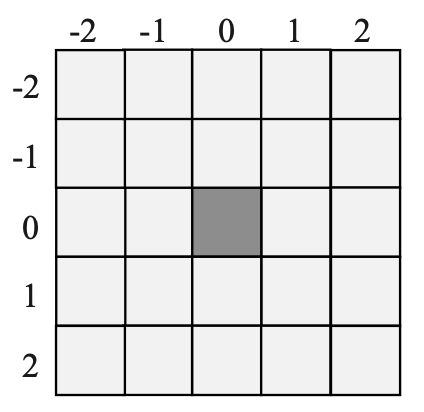
\includegraphics[width=0.60\textwidth]{img/lokaler_operator_maske.jpg}
	\captionof{figure}{Maske eines lokalen Operators nach \citet[S.~52]{handels2000}}
	\label{fig:lokaler_operator_maske}
\end{minipage}

Für die konkrete Betrachtung der Nachbarschaft eines Pixels empfiehlt \citet[S.~52]{handels2000}
eine Maske (Ausschnitt) heranzuziehen, die mit einer Matrix interpretiert werden
kann und die Nachbarschaft eines Pixels abbildet. Abbildung \ref{fig:lokaler_operator_maske}
zeigt eine solche Maske und soll das Verfahren so verdeutlichen. Der grau
hinterlegte Mittelpunkt $P = (0/0)$ ist das aktuell betrachtete Pixel. Die Felder
um die Mitte herum die Nachbarn. Es fällt jedoch auf, dass durch dieses Schema nicht
jede mögliche Ausprägung einer Maske infrage kommt. Um einen Mittelpunkt und
damit ein aktuelles Pixel betrachten zu können, bedarf es eines ungeraden Grades
für $M$. Diese Eingrenzung lässt sich in Gleichung \ref{equ:lokaler_operator}
generisch fassen.

\begin{align}
	\label{equ:lokaler_operator}M_{(2_m+1)x(2_m+1)} & = \begin{bmatrix}k_{11}&k_{12}&k_{13}\\ k_{21}&x&k_{23}\\ k_{31}&k_{32}&k_{33}\\\end{bmatrix} & m \in \mathbb{N}
\end{align}

Die Gleichung \ref{equ:lokaler_operator} beschreibt die mögliche Ausprägung eines
lokalen Operators als Matrix. Dabei sei: $m \in \mathbb{N}\wedge n \in \mathbb{N}$.
Die Variable $x$ beschreibt das aktuell betrachtete Pixel, während $k_{nn}$ die Nachbarn
illustrieren soll. Durch die Gleichung ist auch zu erkennen, dass die Maske des lokalen
Operators beliebig groß werden kann. Eine hohe Ordnung der Operatormatrix ist
jedoch nicht immer von Vorteil, sodass es letzten Endes auf den Anwendungsfall ankommt.

Mit der Technik der lokalen Operatoren können nun unterschiedliche Arten angewendet
werden. \citet[S.~54 - 55]{handels2000} unterscheidet hier in Glättungsfilter,
Mittelwertfilter, Medianfilter, Gaußfilter und Binomialfilter. Alle dieser Filter
bedienen sich einer Operatormaske, um auf Basis der Nachbarelemente einen
statistischen Wert für den Bildpunkt zu erhalten. Um einen genaueren Einblick in
alle Filter zu erlangen, sei an dieser Stelle auf \citet[S.~54 - 55]{handels2000}
verwiesen.

Wie zu Anfang dieses Kapitels beschrieben, ist eine Bildvorverarbeitung (Filterung)
für eine gute Segmentierung des Bildes unerlässlich. So kommt es das auch in der
Visualisierungspipeline nach \citet[S.~50]{handels2000} der zweite Schritt
bereits die Segmentierung einführt. Warum dies so ein wichtiger Bestandteil der Bildanalyse
ist und welche Methoden sich hier bieten, erläutert das folgende Kapitel.
% ---------------------------------------------------------------------------------------

\pagebreak

\subsection{Segmentierung}
\label{subsec:segmentierung} Die Bildsegmentierung oder auch Bildaufteilung genannt,
ist ein wichtiges Teilgebiet der Bildverarbeitung und beschäftigt sich mit der
Bildanalyse. Ihr Ziel ist es, detaillierte beschreibende Bilder aus dem
vorliegenden Originalbild zu berechnen. Dies kann im Falle eines \ac{CT}s der Zahnklinik
an der \ac{LMU} die hervorgehobene Darstellung der Zahnsubstanzen Schmelz und
Dentin sein. \citep[vgl.][S.~359]{lehmann2013bildverarbeitung}. Konkret teilt ein
Segmentierungsverfahren also ein Bild in Teilbereiche auf. Dabei sind die
Teilbereiche in sich bemerkenswert homogen. \citet[S.~1]{ramesh2021} beschreiben,
dass der Prozess der Segmentierung zur Gewinnung wichtiger Informationen dient wie
zum Beispiel die Zahnkaries Ausbreitung. So kommt es, dass \citet[S.~50]{handels2000}
in seiner Visualisierungspipeline die Segmentierung als zweiten Schritt und
damit als zentrales Problem darstellt. \citet[S.~95]{handels2000} und \citet[S.~360]{lehmann2013bildverarbeitung}
beschreiben beide, dass die Bildsegmentierung eines \ac{CT}s für eine gute und
eindeutige ärztliche Diagnose nicht mehr wegzudenken ist. Warum dem so ist,
verdeutlicht die Abbildung \ref{fig:interpretation_einer_ct_aufnahem}.

\begin{figure}[h]
	\centering
	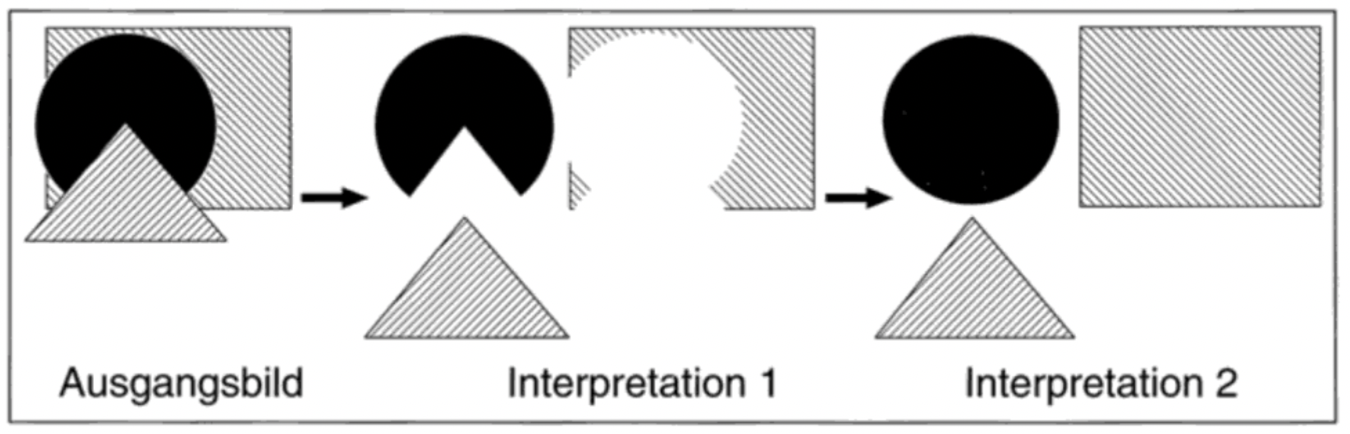
\includegraphics[width=0.8\textwidth]{img/bild_interpretation.jpg}
	\caption{Interpretation einer CT-Aufnahme nach \citet[S.~360]{lehmann2013bildverarbeitung}}
	\label{fig:interpretation_einer_ct_aufnahem}
\end{figure}

Zu erkennen ist das originale Bild (Ausgangslage) und mögliche Interpretationsschritte
(Interpretation 1 und Interpretation 2). \citet[S.~360]{lehmann2013bildverarbeitung}
verdeutlichen mit dieser Abbildung \ref{fig:interpretation_einer_ct_aufnahem},
dass mittels Segmentierung die einzig mögliche Interpretation die Erste ist. Auch
wenn die zweite Interpretation die deutlich logischere ist, kann diese ohne
weitere Forschung nicht bewiesen werden, so \citet[S.~360]{lehmann2013bildverarbeitung}.
Außerdem ist zu erkennen, dass die Abbildung
\ref{fig:interpretation_einer_ct_aufnahem} die Definition einer Segmentierung
belegt. Die Erzeugung inhaltlich zusammengehöriger Regionen werden hier durch die
verschiedenen Formen visualisiert \citep[vgl.][S.~360]{lehmann2013bildverarbeitung}.

Um ein Bild zu segmentieren, gibt es unzählige Möglichkeiten. Für die Auswahl
eines Verfahrens spielt unter anderem der Anwendungsbereich eine wichtige Rolle.
Die Verfahren, die in dieser Arbeit von Wichtigkeit sind, sind die Schwellwertverfahren
\citep[vgl.][S.~361]{lehmann2013bildverarbeitung}.

\pagebreak

\textbf{Schwellwertverfahren} (engl.: thresholding) gehören zu den
Standardwerkzeugen einer Segmentierung, sodass diese die Basis vieler weiterer Verfahren
legen. Bei einer schwellwertbasierten Segmentierung werden die Pixel eines
Bildes anhand von Schwellwerten eingruppiert \citep[vgl.][S.~96]{handels2000}.
Die nachfolgende Gleichung \ref{equ:schwellwertverfahren} soll dies
verdeutlichen.

\begin{align}
	\label{equ:schwellwertverfahren}B(x, y, z) = \begin{cases}1,&\text{falls }t_{\text{unten}}\leq f(x, y, z) \leq t_{\text{oben}}, \\ 0,&\text{sonst}.\end{cases}
\end{align}

$B(x, y, z)$ beschreibt ein Pixel in einem dreidimensionalen Bild, demnach ein
Voxel. Liegen die Werte eines Voxels, also $f(x, y, z)$, innerhalb der beiden Schwellwerte
$t_{oben}$ und $t_{unten}$, dann wird eine 1 zugewiesen. Liegt der aktuell betrachtete
Voxel nicht zwischen den Schwellwerten, so wird eine 0 zugewiesen. Das Ergebnis einer
solchen primitiven Schwellwertsegmentierung ist ein binäres Bild, welches in
Abbildung \ref{fig:binäres_schwellwertverfahren} zu sehen ist.

\begin{figure}[h]
	\centering
	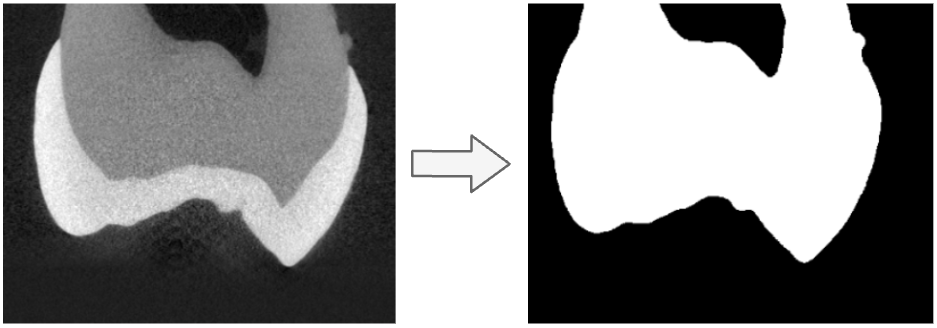
\includegraphics[width=0.8\textwidth]{img/beispiel_schwellwertverfahren.png}
	\caption{Ergebnis eines einfachen Schwellwertverfahrens nach \citet{heck2024} und
	\citet{hoffmann2020}}
	\label{fig:binäres_schwellwertverfahren}
\end{figure}

Zu erkennen ist, dass nach einem einfachen Schwellwertverfahren das Bild nur
noch aus zwei unterschiedlichen Graustufen besteht. Betrachtet man das Ergebnis in
\ref{fig:binäres_schwellwertverfahren} genauer, so ist diese einfache
Segmentierung durchaus erfolgreich verlaufen. Der Grund dafür ist die gute Wahl des
Schwellwerts.

Die interessanteste Frage bei den Schwellwertverfahren ist die Wahl des Schwellwerts
$t$. Dieser entscheidet zwischen einer guten und einer schlechten Segmentierung.
Für die Wahl eines Schwellwerts empfiehlt sich der Blick auf das Bildhistogramm.
Dieses gibt Aufschluss über die Verteilung der Grauwerte in einem Bild \citep[vgl.][S.~361]{lehmann2013bildverarbeitung}.
Verfahren, welche einen guten Schwellwert gewährleistet, ohne dass zu viele
Informationen verloren gehen, sind die Verfahren \textit{Otsu} und \textit{Renyi}.

\pagebreak

\textbf{Das Verfahren nach Otsu} gehört zu den Schwellwertverfahren und bestimmt
den Schwellwert $t$ durch ein statistisches Gütekriterium. Hierzu bedient sich
das Verfahren des Bildhistogramms. Die räumliche Anordnung der Voxel und damit das
tatsächliche Bild, benötigt dieser Algorithmus nicht \citep[vgl.][S.~264]{lehmann2013bildverarbeitung}.

\begin{minipage}{0.40\textwidth}
	Ein solches Histogramm, welches die Grundlage für das Verfahren nach Otsu
	liefert, sei in Abbildung \ref{fig:histogramm} gezeigt. Dies gibt Aufschluss
	über die unterschiedlichen Grauwerte und wie oft sie in einem Bild vorkommen
	\citep[vgl.][S.~264]{lehmann2013bildverarbeitung}. Für eine genauere
	Beschreibung eines Histogramms sei an dieser Stelle auf \citet[S.~42]{burger2009}
	verwiesen.
\end{minipage}
\hfill
\begin{minipage}{0.50\textwidth}
	\centering
	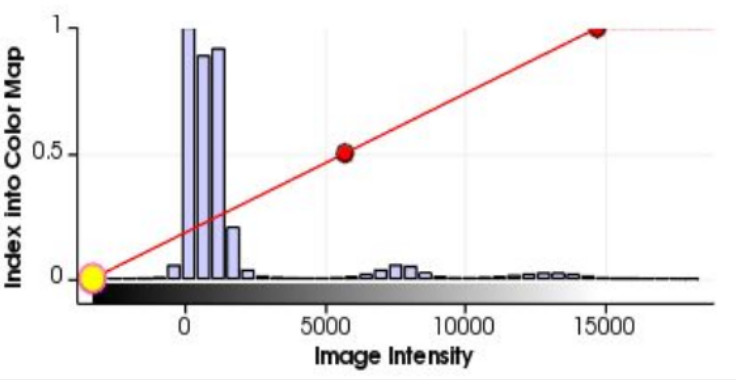
\includegraphics[width=1\textwidth]{img/histogramm.jpg}
	\captionof{figure}{Histogramm einer CT-Aufnahme einer Zahnkrone nach \citet[S.~13]{hoffmann2020}}
	\label{fig:histogramm}
\end{minipage}

Das Otsu-Verfahren teilt die Grauwerte eines Bildes in verschiedenen Klassen ein,
die durch Schwellwerte getrennt werden. Die Klassen können beispielsweise mit
$K_{0}$ bis $K_{n}$ bezeichnet werden, wobei sich dieses konkrete Beispiel auf die
Klassen $K_{0}$ und $K_{1}$ beschränkt. Otsu wählt den Schwellwert $t$, der die Varianz
zwischen den Pixelklassen maximiert und gleichzeitig die Varianz innerhalb jeder
Klasse minimiert \citep[vgl.][S.~264]{lehmann2013bildverarbeitung}. Mathematisch
lässt sich dies wie folgt ausdrücken.
\begin{align}
	t = \text{max }(\sigma_{zw}^{2}/ \sigma_{in}^{2})
\end{align}
$\sigma_{zw}$ bildet die Varianz zwischen den beiden Klassen $K_{0}$ und $K_{1}$
und bildet sich aus den Wahrscheinlichkeiten, mit denen jeder einzelne Grauwert auftritt.
$\sigma_{in}$ hingegen, ist die Varianz innerhalb einer Klasse und entsteht durch
die Addition der Varianzen der einzelnen Klassen. Der Schwellwert $t$ ist nun
der, für den das Verhältnis maximal wird \citep[vgl.][S.~264]{lehmann2013bildverarbeitung}.

Laut \citet[S.~264]{lehmann2013bildverarbeitung} fällt auf, dass dieses
Verfahren vor allem bei bimodalen Bildern zum Einsatz kommt. Ein Bild ist bimodal,
wenn es zwei lokale Maxima aufweist. Vereinfacht gesagt, wenn es zwei lokale
Piecks enthält \citep[vgl.][S.~264]{lehmann2013bildverarbeitung}.

Eine ähnliche Technik für die Bestimmung des Schwellwerts liefert das Verfahren der
Rényi Entropie. Auch hier ist eine Einteilung der Voxel in Klassen vorgesehen.

\pagebreak
% ---------------------------------------------------------------------------------------

\textbf{Das Verfahren nach Rényi} ist ein weiteres Verfahren, das im Laufe dieser
Arbeit noch eine wichtige Rolle spielt. Wie bereits beschrieben gehört es
ebenfalls zu der Gruppe der Schwellwertverfahren und generiert demnach einen
Schwellwert $t$. Wie auch das Verfahren nach Otsu, benötigt Rényi keine
Information über die räumliche Anordnung der Bilder, es genügt das Bildhistogramm.
Dabei ist der optimal Schwellwert $t$ der, der eine maximale Entropie der Bildverteilung
erzeugt. Unter einer Entropie wird ein Konzept verstanden, das eine Unordnung,
Unsicherheit oder den Informationsgehalt innerhalb eines Systems beschreibt, so \citet[S.~102]{bein2006}.
Die Rényi-Entropie ist eine Verallgemeinerung der Shannon-Entropie und hängt von
einem Parameter $q$ ab. Die Entropie misst die Unsicherheit oder den
Informationsgehalt einer Wahrscheinlichkeitsverteilung, welche sich wie folgt ausdrücken
lässt. \citep[vgl.][K.~2]{bromiley2004}.
\begin{align}
	\label{equ:renyi}H_{q}(P) = \frac{1}{1-q}\ln \left( \sum_{i=1}^{N}p_{i}^{q}\right)
\end{align}
Besonderes Augenmerk verdienen hierbei die Parameter $p_{i}$ und $q$, welche die
charakteristischen Eigenschaften der Rényi-Entropie beschreiben. Der Parameter
$p_{i}$ ist die Wahrscheinlichkeit eines jeden Grauwertes im Bild. $i$ symbolisiert
hierbei jeden Grauwert. Wie viele Grauwerte genau betrachten werden sollen
definiert $N$. Die Variable $q$ hingegen beeinflusst die Gewichtung der Wahrscheinlichkeit
$p_{i}$ für jeden Grauwert. Setzt man den Parameter $q$ auf $q = 1$ so lässt
sich mittels Algebra die Shannon-Entropie zeigen \citep[vgl.][K.~2]{bromiley2004}.
Um nun mit der Rényi-Entropie den optimalen Schwellwert für ein Bild zu
berechnen, sieht Rényi ähnlich wie Otsu eine Einteilung in Klassen vor. Die
Einteilung erfolgt mittels des Parameters $N$. So kann nun für jede gebildete Klasse
die Gleichung \ref{equ:renyi} angewendet werden. Die Gesamtentropie des Systems
wird aus den beiden Teilentropien der jeweiligen Klassen bestimmt\citep[vgl.][K.~2]{bromiley2004}.
\begin{align}
	H_{q}(T) = H_{q}(P)^{(1)}+ H_{q}(P)^{(2)}
\end{align}
Um nun den optimalen Schwellwert $t$ bestimmen zu können muss der Wert genommen werden,
bei dem die Gesamtentropie des Systems maximal ist. Dieser Sachverhalt lässt sich
wie folgt ausdrücken \citep[vgl.][K.~2]{bromiley2004}.
\begin{align}
	t = max(H_{q}(T))
\end{align}
Gegen Ende des Kapitels konnte ein grundlegendes Verständnis über die anatomische
Segmentierung einer Zahn-\ac{CT}-Aufnahme gewonnen werden. Um dieses Verfahren,
wie von der Fragestellung gefordert, für den klinischen Alltag zugänglich zu machen,
ist eine benutzerfreundliche Lösung erforderlich. Im folgenden Kapitel wird daher
die automatische Segmentierung mit 3D Slicer behandelt, einer etablierten
Plattform, die eine effiziente Integration und Nutzung des Verfahrens ermöglicht.
% ---------------------------------------------------------------------------------------